\documentclass{article}

\usepackage{graphicx}
\begin{document}

\title{STAT 159/259 Project proposal }
\author{
  Jo, Min Gu\\
  \texttt{mingujo}
  \and
  Kaam, Soazig\\
  \texttt{soazig}
  \and
  Li, Zhuangdi\\
  \texttt{lizhua}
  \and
  Yu, Timothy\\
  \texttt{github3}
  \and
  Zhi, Ye\\
  \texttt{ye-zhi}
  }

\maketitle


\section{Background and methods}
\noindent
Previous studies investigated the brain activity related to the the anticipation or the experience of gaining or losing money. The present study focuses on decision-making process, especially the correlation between the neural activity and the reluctance to lose.\\\\
16 people were presented gambling situations with a 50\% of success. Each situation was associated with a potential gain and loss that were randomly selected. The gains were ranging from \$10 to \$40 while the losses from \$5 to \$20. To allow flexibility in the decision making, answers from participants were collected using likert scales. For each case, one of the following will reflect the most the participant choice of taking or not the gamble: strongly accept, weakly accept, weakly reject, strongly reject. The response time was also recorded for each case. \\\\
The imaging data were collected using the fMRI method. They were processed and analyzed in order to identify the regions of the brain activated by the decision making process. This study also investigated the relationship between the brain activity and the behavior of the subjects towards the gambling situations. 


\section{Results}
This study was able to identify gain-sensitive areas in the brain that showed an increasing or decreasing activity depending on potential loss or gain. It successfully identified the regions that were related to decision utility. The study showed that there was no significant difference in the imaging, comparing the activity for the best and the worst possible gamble.\\\\
These results were consistent with previous studies on the topic, which demonstrated that the same brain mechanism was involved in losses and gains. They observed bidirectional activities (increasing and decreasing) in the same regions.\\\\
As expected, results show the probability of acceptance is higher for a high gain and low loss combination. In addition, the response time is faster for a decision involving high gain/low loss or low gain/high loss. On the other hand, they observed slower time response for cases with medium potential gain or loss, where the situation presented leads to a decision that needs more reflexion for the subject.\\\\
The study showed that the behavior, i.e the actual response of the participant to the survey, and the brain activity were strongly correlated.  For the majority of the participants, they associated a decrease in loss aversion with a decrease in neural activity. The results support the common hypothesis that the brain is more sensitive to losses than gains. Besides, each subject had different sensitivity regarding potential loss, which is the primary driver to  decision making.




\section{Data Sanity Check}
\noindent
We could confirm that the download raw data file contains demographic information(age and gender of participants), 16 data folders (each folder for each of 16 participants), and license information, etc. Each data folder contains the subject?s anatomy, behavioral data, BOLD image data, and model (participant?s behavioral model of decision making under risk and uncertainty). Anatomy data contains the subject?s brain image. Behavioral data illustrates the behavioral sensitivity to gains and losses recorded by participants for each trial of gambling situations with different gain and loss amount. BOLD image data is the observation done by the researchers. Model is the behavioral sensitivity model fitted by a logistic regression to each participant?s acceptability judgments collected during scanning. Since the test was run 3 times on each participant, there are 3 sets of each behavioral, BOLD, and model. \\\\
\noindent
Sample Image : the BOLD image of test 2 of Subject 1. 
\begin{figure}[h]
\centering
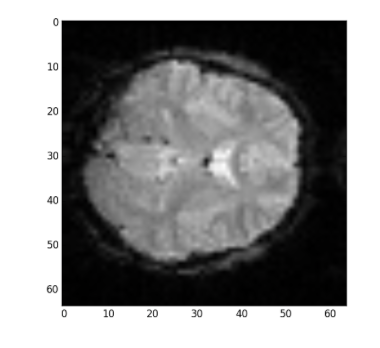
\includegraphics[width=0.3\columnwidth]{sampleimage}

\end{figure}



\section{Our approach:}
\noindent
First we need to identify the regions of the brain which activity are related to decision making process. We will use the same method of finding brain activation using BOLD data as shown in class, and then compare with the regions they found. We also need to consider amount of money gain/loss ratio with activity of the brain.\\\\
Secondly, we use logistic regression to relate gain to loss ratio to the activity of the regions of the brain related to the decision making process . The study showed we would be more likely to take a risk if the gain is twice as important as the gain. We will try to confirm these results with the analysis by looking at the gain to loss ratio the case and see if we can use machine learning techniques (logistic regression) to predict the decision made by the subject.\\\\
In order to get a binary model choice, we will preprocess the likert scale as follow: strongly accept + weekly accept $\Rightarrow$ accept and weekly reject + strongly reject $\Rightarrow$ reject
We can also try a multiple choice mode with 4 levels and keep the likert scale as is.\\\\
Finally, we will also investigate Gender/Age influence on decision making process




\end{document}


